
%(BEGIN_QUESTION)
% Copyright 2010, Tony R. Kuphaldt, released under the Creative Commons Attribution License (v 1.0)
% This means you may do almost anything with this work of mine, so long as you give me proper credit

This is an electronic thermal conductivity sensor, used to detect different chemical components exiting the column of a chromatograph.  Both the measurement and reference filaments are heated by the electric current going through them, and a varying voltage will develop across each one as each is cooled differently by the gases:

$$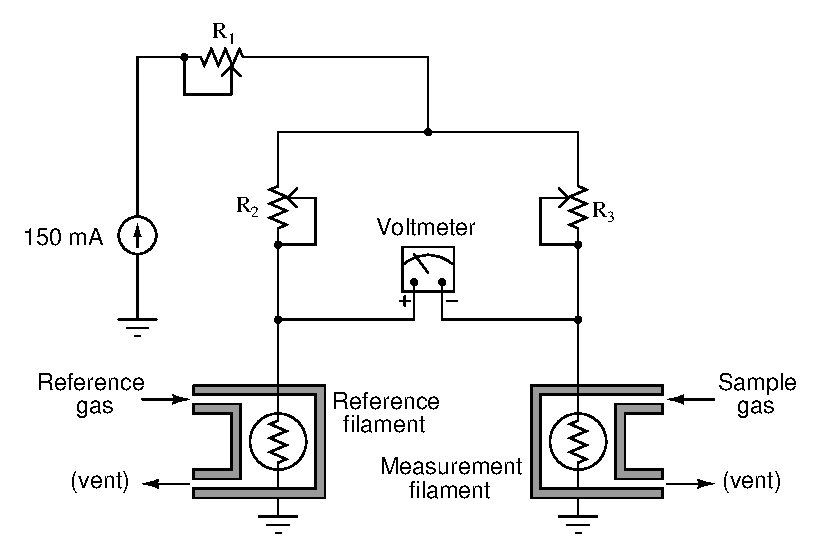
\includegraphics[width=15.5cm]{i00909x01.eps}$$

Suppose a technician is setting up this detector for the very first time, and notes the voltmeter registers an abnormally large signal (in the polarity shown) even with the same test gas passed through each cell.

Identify the likelihood of each specified fault for this circuit.  Consider each fault one at a time (i.e. no coincidental faults), determining whether or not each fault could independently account for {\it all} measurements and symptoms in this circuit.

% No blank lines allowed between lines of an \halign structure!
% I use comments (%) instead, so that TeX doesn't choke.

$$\vbox{\offinterlineskip
\halign{\strut
\vrule \quad\hfil # \ \hfil & 
\vrule \quad\hfil # \ \hfil & 
\vrule \quad\hfil # \ \hfil \vrule \cr
\noalign{\hrule}
%
% First row
{\bf Fault} & {\bf Possible} & {\bf Impossible} \cr
%
\noalign{\hrule}
%
% Another row
$R_1$ resistance set too low &  &  \cr
%
\noalign{\hrule}
%
% Another row
$R_1$ resistance set too high &  &  \cr
%
\noalign{\hrule}
%
% Another row
$R_2$ resistance set too low &  &  \cr
%
\noalign{\hrule}
%
% Another row
$R_2$ resistance set too high &  &  \cr
%
\noalign{\hrule}
%
% Another row
$R_3$ resistance set too low &  &  \cr
%
\noalign{\hrule}
%
% Another row
$R_3$ resistance set too high &  &  \cr
%
\noalign{\hrule}
%
% Another row
Reference filament burned open &  &  \cr
%
\noalign{\hrule}
%
% Another row
Measurement filament burned open &  &  \cr
%
\noalign{\hrule}
%
% Another row
Voltmeter failed open &  &  \cr
%
\noalign{\hrule}
%
% Another row
Voltmeter failed shorted &  &  \cr
%
\noalign{\hrule}
} % End of \halign 
}$$ % End of \vbox


\underbar{file i00909}
%(END_QUESTION)





%(BEGIN_ANSWER)

% No blank lines allowed between lines of an \halign structure!
% I use comments (%) instead, so that TeX doesn't choke.

$$\vbox{\offinterlineskip
\halign{\strut
\vrule \quad\hfil # \ \hfil & 
\vrule \quad\hfil # \ \hfil & 
\vrule \quad\hfil # \ \hfil \vrule \cr
\noalign{\hrule}
%
% First row
{\bf Fault} & {\bf Possible} & {\bf Impossible} \cr
%
\noalign{\hrule}
%
% Another row
$R_1$ resistance set too low &  & $\surd$ \cr
%
\noalign{\hrule}
%
% Another row
$R_1$ resistance set too high &  & $\surd$ \cr
%
\noalign{\hrule}
%
% Another row
$R_2$ resistance set too low & $\surd$ &  \cr
%
\noalign{\hrule}
%
% Another row
$R_2$ resistance set too high &  & $\surd$ \cr
%
\noalign{\hrule}
%
% Another row
$R_3$ resistance set too low &  & $\surd$ \cr
%
\noalign{\hrule}
%
% Another row
$R_3$ resistance set too high & $\surd$ &  \cr
%
\noalign{\hrule}
%
% Another row
Reference filament burned open & $\surd$ &  \cr
%
\noalign{\hrule}
%
% Another row
Measurement filament burned open &  & $\surd$ \cr
%
\noalign{\hrule}
%
% Another row
Voltmeter failed open &  & $\surd$ \cr
%
\noalign{\hrule}
%
% Another row
Voltmeter failed shorted &  & $\surd$ \cr
%
\noalign{\hrule}
} % End of \halign 
}$$ % End of \vbox


%(END_ANSWER)





%(BEGIN_NOTES)

$$\includegraphics[width=15.5cm]{i00909x02.eps}$$

\vskip 20pt \vbox{\hrule \hbox{\strut \vrule{} {\bf Virtual Troubleshooting} \vrule} \hrule}

This question is a good candidate for a ``Virtual Troubleshooting'' exercise.  Presenting the diagram to students, you first imagine in your own mind a particular fault in the system.  Then, you present one or more symptoms of that fault (something noticeable by an operator or other user of the system).  Students then propose various diagnostic tests to perform on this system to identify the nature and location of the fault, as though they were technicians trying to troubleshoot the problem.  Your job is to tell them what the result(s) would be for each of the proposed diagnostic tests, documenting those results where all the students can see.

During and after the exercise, it is good to ask students follow-up questions such as:

\begin{itemize}
\item{} What does the result of the last diagnostic test tell you about the fault?
\item{} Suppose the results of the last diagnostic test were different.  What then would that result tell you about the fault?
\item{} Is the last diagnostic test the best one we could do?
\item{} What would be the ideal order of tests, to diagnose the problem in as few steps as possible?
\end{itemize}


%INDEX% Measurement, analytical: chromatography
%INDEX% Troubleshooting review: electric circuits

%(END_NOTES)


